
\chapter{The Eletronics} \label{chap:electronics}

In order for the aircraft to fly and navigate autonomously, onboard electronics are required, for both actuation, power source, and navigation. Some of the used electronics were already available, and were chosen for this reason.
	
\section{Propulsion}

Due to the familiriaty and availability, the Mikrokopter Mk3538 Motor was chosen, paired with E-Max Simon 60A escs.

Experimental curves for the motor are available at Mikrokopter's website, and the relevant ones are reproduced on Figure \ref{fig:motorcurves}. Each motor should give, on 25 V, at least 2.2kg of static thrust when paired to 12 inches propellers, up to 3.4 kg on 15 inches, while drawing 34 A, or about 754 W.
\begin{figure}
\centering
  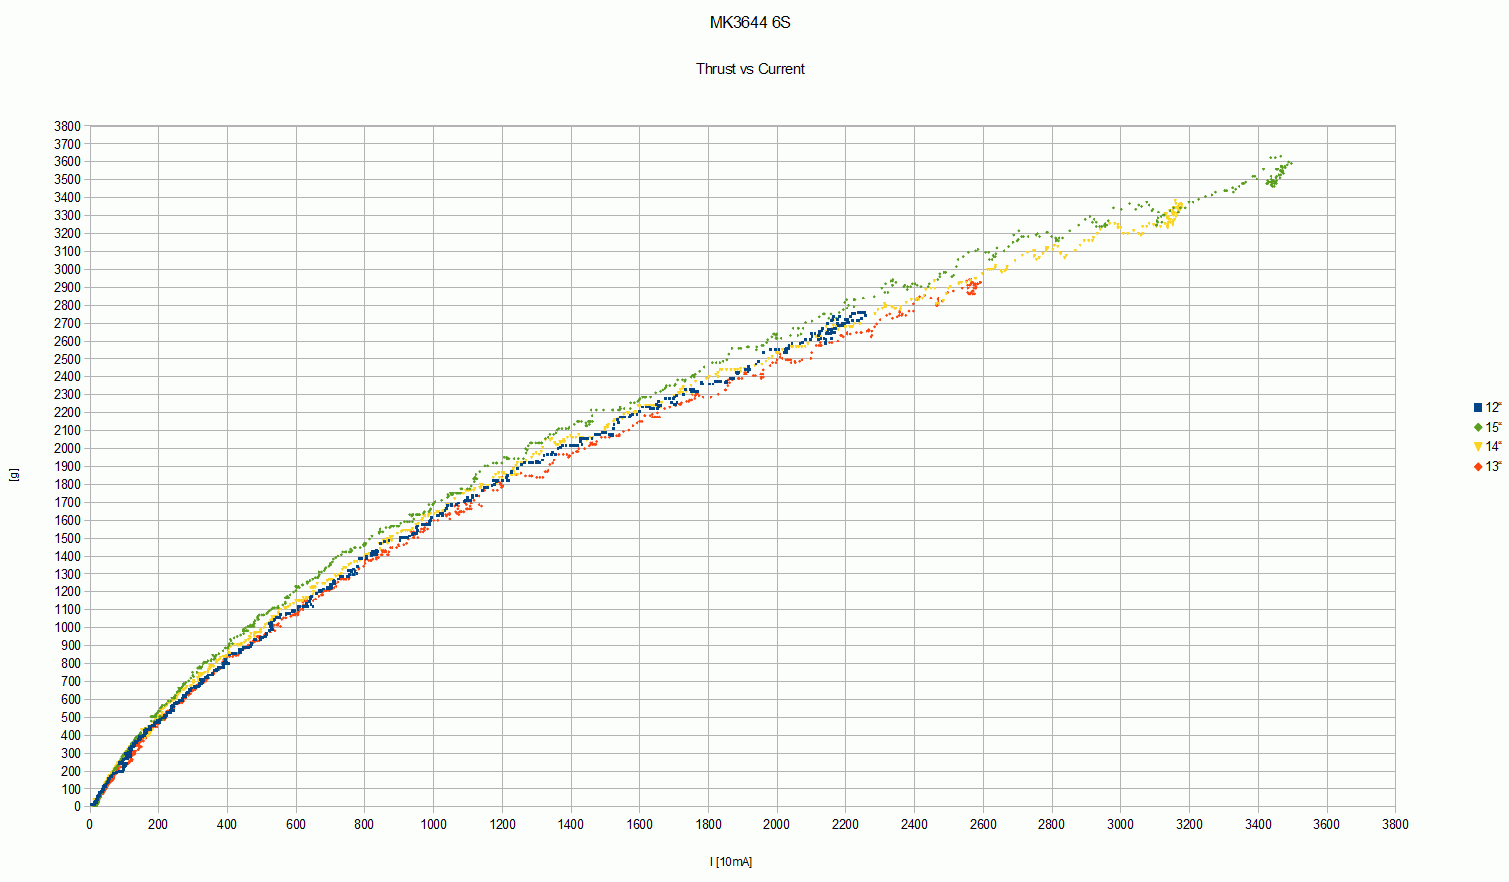
\includegraphics[width=\linewidth]{figs/motorcurves.png}
  \caption{First concept of the aircraft.}
  \label{fig:motorcurves}
\end{figure}


\section{Batteries}

As each motor can draw up to 34 A, the battery should be able to provide up to 68 A without issues.
The Batteries chosen are also the ones already in use by the company, Vislero 4500 mAh 20C, which, at 20 C rating, are able to sustain a constant draw of up to 90 A. 

Each weigh approximately 750 g and measures XXxYYxZZ mm.

\section{The Control Surfaces}

The control surfaces must be slightly larger than usual for a flying wing, as on a tail-sitter a reasonable amount of air must be deflected on hover situation, while on most wings a steady airflow is assumed. It's suggested to have control surfaces taking up to 30\% of the chord of the wings. Since they are easily swappable, it was decided to start with smaller ones, and replace it if necessary

\section{The Flight Controller}

The multirotor had a huge boom last 10 years. In 2009 the first hobby-grade flight controller for multicopters was born, Rolf “KaptainKuk” Bakke's "KK board". Using a simple AVR controller and three gyroscopes, the board could control angular speed on three axis, enabling pilots to control the multirotors. It was programmed in AVR assembly and had individual PID controllers for each axis.
%
Shortly after, Alexinparis noticed the gyros on the Wii Motion + controller, and MultiWii was born. This project grew to support a variety of sensors and boards, and had an active development community, but has now saturated the AVR controller's capability.
%
Shortly after, still in 2010, DIY Drones released the open-source Arducopter, featuring more advanced flight modes, and even autonomous flight.  It did still involve compiling code and flashing it to the controller though.
%
In 2011, DJI started to get visibility with the NAZA controller, which showed remarkable stability, and later got upgraded with a GPS allowing the drone to return to home and hold position in the air. The controller was often sold with a 





The Flight Controller is a PixHawk, running latest Beta release of ArduPlane, where there's experimental support for tail-sitters.


%%%%%%%%%%%%%%%%%%%